\chapter{Introduction}

\begin{remark}{Outline}
\todo{outline}
In this chapter, we present the well-known family of \textit{random forests}
methods. In Section~\ref{sec:4:bias-variance}, we first describe the bias-variance
decomposition of the prediction error and then present, in
Section~\ref{sec:4:ensemble}, how aggregating randomized models through
ensembles reduces the prediction error by decreasing the variance term in this
decomposition. In Section~\ref{sec:4:random-forests}, we revisit random forests
and its variants and study how randomness introduced into the decision trees
reduces prediction errors by decorrelating the decision
trees in the ensemble. Properties and features of random forests are then outlined
in Section~\ref{sec:4:features} while their consistency
is finally explored in Section~\ref{sec:4:consistency}.
\end{remark}


\section{Classification models}
In machine learning, classification refers to the attempt of identifying to which of a set of 
classes a new example belongs, based on learning from examples whose class membership is known. 
The most important point about classification is that for each example only one know class is 
possible, making this a discrete problem. 


\chapter{Background}

\begin{remark}{Outline}
\todo{outline}
In this chapter, we present the well-known family of \textit{random forests}
methods. In Section~\ref{sec:4:bias-variance}, we first describe the bias-variance
decomposition of the prediction error and then present, in
Section~\ref{sec:4:ensemble}, how aggregating randomized models through
ensembles reduces the prediction error by decreasing the variance term in this
decomposition. In Section~\ref{sec:4:random-forests}, we revisit random forests
and its variants and study how randomness introduced into the decision trees
reduces prediction errors by decorrelating the decision
trees in the ensemble. Properties and features of random forests are then outlined
in Section~\ref{sec:4:features} while their consistency
is finally explored in Section~\ref{sec:4:consistency}.
\end{remark}


\section{Basics on classification}
In machine learning, classification refers to the attempt of identifying to which of a set of 
classes a new example belongs, based on learning from examples whose class membership is known. 
The most important point about classification is that for each example only one know class is 
possible, making this a discrete problem. 

A classification, task begins with a training set in which the class of a set of examples is know. 
For example, a classification model that predicts credit card fraud, is developed by analyzing 
many observed credit transactions over a period of time. The class in this case is a variable which 
indicates for each example whether or not the transaction was o not a fraud. Also, the predictors 
or features, are the transaction attributes like place, amount and time of the transaction.

Then, during the training process, a classification algorithm finds the patterns and relationships 
between the values of the features and the values of the target class. Different algorithms use 
different methods and techniques to estimate the relationships. Afterwards, these relationships are 
summarized in a model that is able to make predictions on new sets of data.

Formally, a classification algorithm deals with the problem	of predicting the class $y_i$ of a 
set $\cal S$ of examples or instances, given their $k$ features \mbox{$\bf{X}_i \in 
\mathbb{R}^k$}. The objective is to construct a function $f(\cal{S})$ that makes a prediction 
$c_i$ of the class of each of the $N$ examples using its feature vector $\bf{X}_i$.
\label{ntn:ch2:1}

\begin{figure}
	\centering
	  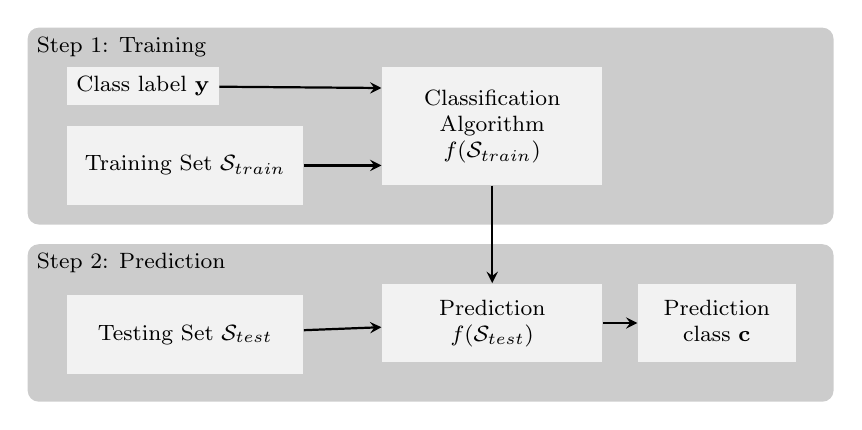
\begin{tikzpicture}[node distance=2cm]
  \tikzstyle{every node}=[font=\footnotesize]
  
  % Main boxes
  \node (step1) [rectangle, rounded corners, anchor=north west, fill=black!20, text width=10cm,
								minimum height=2.5cm] {};
	\node [anchor=north west] at (step1.north west){Step 1: Training};
	\node (step2) [rectangle, rounded corners, anchor=west, fill=black!20, text width=10cm, 
								minimum height=2cm, below of = step1, yshift=-0.5cm] {};
	\node [anchor=north west] at (step2.north west){Step 2: Prediction};
	
	% Training
	\node (label) [rectangle, anchor=north west, fill=black!5,
								yshift=-0.5cm, xshift=0.5cm] {Class label $\bf y $};
	\node (train) [rectangle, anchor=north west, fill=black!5, minimum height=1cm, minimum width=3cm,
								yshift=-1.25cm, xshift=0.5cm] {Training Set $\mathcal{S}_{train} $};
	\node (algo) [rectangle, anchor=north west, fill=black!5, minimum height=1.5cm,
							 minimum width=2.8cm, yshift=-.50cm, xshift=4.5cm] 
							 {\tabular{c} Classification \\ Algorithm  \\	$f(\mathcal{S}_{train}) $
								\endtabular}; 

	%Classification
	\node (test) [rectangle, anchor=north west, fill=black!5, minimum height=1cm, minimum width=3cm,
								yshift=-3.4cm, xshift=0.5cm] {Testing Set $\mathcal{S}_{test} $};
	\node (algo2)[rectangle, anchor=north west, fill=black!5, minimum height=1cm, minimum width=2.8cm,
							 yshift=-3.25cm, xshift=4.5cm] 
							 {\tabular{c} Prediction \\	$f(\mathcal{S}_{test}) $\endtabular};
	\node (pred) [rectangle, anchor=north west, fill=black!5, minimum height=1cm,
							yshift=-3.25cm, xshift=7.75cm] {\tabular{c} Prediction \\ class $\bf c$	\endtabular};
	
	% Arrows
	\node (label_temp) [rectangle, anchor=north west, yshift=-0.65cm, xshift=4.5cm] {};
	\draw[thick,->,>=stealth] (label) to (label_temp);
	\node (train_temp) [rectangle, anchor=north west,minimum height=1cm, minimum width=3cm,
								yshift=-1.25cm, xshift=4.5cm] {};
	\draw[thick,->,>=stealth] (train) to (train_temp);
	\draw[thick,->,>=stealth] (algo) to (algo2);
	\draw[thick,->,>=stealth] (test) to (algo2);
	\draw[thick,->,>=stealth] (algo2) to (pred);
  \end{tikzpicture}
 
  \caption{Classification process}
  \label{fig:ch2:0}
\end{figure}

\todo{Change training eq}

In \figurename{ \ref{fig:ch2:0}}, the process of a training and using a classification algorithm is 
summarized. First, during the training phase, using a training set $\mathcal{S}_{train}$, a 
algorithm is train to predict $\bf y$. Then the algorithm is used to make estimate the class $\bf 
c$ of a set of testing examples $\mathcal{S}_{test}$.

\begin{figure}[!t]
\centering
\subfloat[]{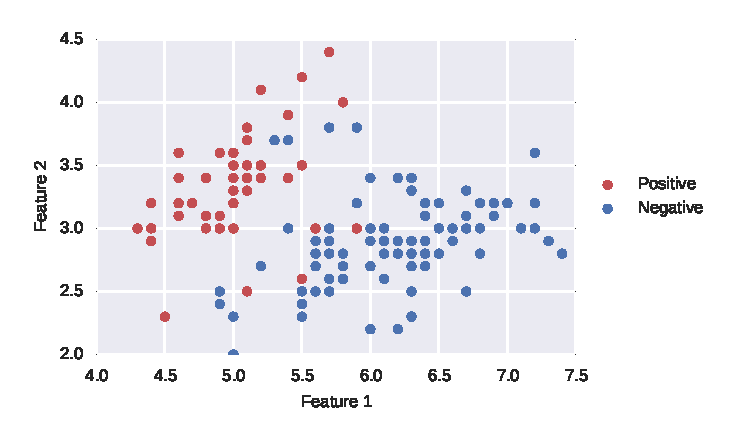
\includegraphics{ch2_fig1a}\label{fig:ch2:1a}}
\\
\subfloat[]{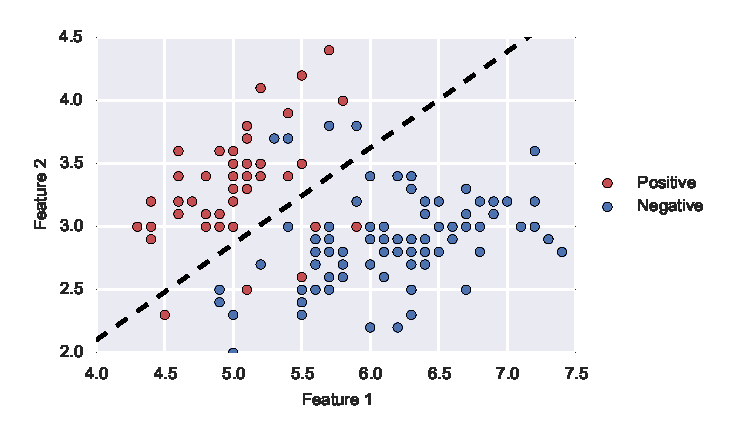
\includegraphics{ch2_fig1b}\label{fig:ch2:1b}}
\caption{Example of a classification algorithm. Using a set of examples from two classes, a 
	classification algorithm is learn in order to separate between the positives and the negatives. }
\label{fig:ch2:1}
\end{figure} 

There exists several algorithms that can be used for classification tasks. In general a 
classification algorithm is learn with the objective of finding patterns that separate between the 
different classes. In order to clarify this intuition, in \figurename{ \ref{fig:ch2:1}} an example 
of a classification algorithm is shown. Lets suppose a set of examples as shown in \figurename{ 
\ref{fig:ch2:1a}}.  Where the red points represents the positive examples and the blue the negative 
examples. The objective of a classifier is to find the best way to separate between the positive and 
negatives examples. In \figurename{ \ref{fig:ch2:1b}}, the output of a classifier learned using the 
set of examples is shown. It is observed that this classifier is able to separate almost all the 
examples using a linear classifier. 

However, not all examples are correctly classified. In particular there are 4 negative examples that 
were predicted as positive, and 5 positive examples that were predicted as negative. In the next 
section, we present the standard methods for evaluating the performance of a classification 
algorithm.

\begin{remark}{Classification examples}
Classification algorithms are widely used across a variety of domains. For example in the 
medical field, models have been used for making predictions about tumors, probability 
of a disease, selecting the right drug for a particular patient, and estimating the probability of 
relapsing, among others \citep{Herland2014}. In the financial sector, classification models have 
been successfully applied for fraud detection, credit scoring, portfolio management and algorithmic 
trading. Also, in marketing, several models are being currently used for churn modeling, customer 
targeting, behavior prediction and direct marketing \citep{Baesens2014}. Additionally, in many 
other emerging applications such as terrorism prevention, malware detection, computer security, 
energy consumption prediction, spam classification, and others \citep{Kriegel2007}.
\end{remark}

\subsection{Performance measures}

When evaluating the performance of a classification algorithm, the first thing to do is to check 
the number of examples that were misclassified. Since the the true class of the training examples 
is known. Therefore, evaluating the error of a model is as simply as counting the number of times 
an example is misclassified and divide it by the number of examples.

\begin{equation}\label{eqn:ch2:error}
Err(f({\cal S})) = \frac{1}{N}  \sum_{i=1}^N {\bf 1} _{y_i}(c_i),
\end{equation}
where $\mathbf{1}_c(z)$ is an indicator function that takes the value of one if $z \in c$ and 
zero if $z \notin c$. Moreover the accuracy is defined as the percentage of times the algorithm 
made the correct prediction
\begin{equation}\label{eqn:ch2:accuracy}
Acc(f({\cal S})) = 1- Err(f({\cal S})).
\end{equation}

However, just knowing these statistics is not enough to make decisions, as in many applications is 
important to know where the errors are coming from. In particular, the misclassified examples may 
belong only to one class, which may give interesting insights about the problem.
A way to observe the different errors is by looking to the confusion matrix.
As shown in \tablename{ \ref{tab:ch2:1}}, 
\todo{how to calculate TP, FP...}

	\begin{table}[!t]
		\centering
		\footnotesize
    \begin{tabular}{c|c|c}
      \multicolumn{3}{c}{}\\
			\multicolumn{1}{c|}{}  & Actual Positive& Actual Negative \\
			\multicolumn{1}{c|}{} & $y=1$& $y=0$ \\
			\hline
			Predicted Positive 		& \multirow{ 2}{*}{True Positive ($TP$)} & \multirow{ 
			2}{*}{False Positive ($FP$)} \\
			$c=1$ & &\\
			\hline
			Predicted Negative  	& \multirow{ 2}{*}{False Negative ($FN$)} & \multirow{ 
			2}{*}{True Positive ($TN$)} \\
			$c=0$ & &\\
		\end{tabular}
		\caption{Classification confusion matrix}
		\label{tab:ch2:1}
  \end{table}  

  	From this table several statistics are extracted. In particular:
	\begin{itemize}
		\item Recall = $\frac{TP}{TP+FN}$
		\item Precision = $\frac{TP}{TP+FP}$
		\item $F_1Score = 2\frac{Precision \cdot Recall}{Precision + Recall}$
	\end{itemize}


  
  	\begin{table}[!t]
		\centering
		\footnotesize
    \begin{tabular}{c|c|c}
      \multicolumn{3}{c}{}\\
			\multicolumn{1}{c|}{}  & Actual Positive& Actual Negative \\
			\multicolumn{1}{c|}{} & $y=1$& $y=0$ \\
			\hline
			Predicted Positive 		& \multirow{ 2}{*}{36} & \multirow{ 
			2}{*}{4} \\
			$c=1$ & &\\
			\hline
			Predicted Negative  	& \multirow{ 2}{*}{5} & \multirow{ 
			2}{*}{68} \\
			$c=0$ & &\\
		\end{tabular}
		\caption{Confusion matrix of the toy example}
		\label{tab:ch2:2}
  \end{table}  
  
  Calculating the different statistics for this example
  	\begin{itemize}
  	\item Error = $\frac{4+9}{36+4+9+68}=8\%$
		\item Recall = $\frac{TP}{TP+FN}$
		\item Precision = $\frac{TP}{TP+FP}$
		\item $F_1Score = 2\frac{Precision \cdot Recall}{Precision + Recall}$
	\end{itemize}
	
	In order to make a comparison, using the same example toy set, a new algorithm is learn. This 
time the algorithm made the correct prediction more often as shown in \figurename{ \ref{fig:ch2:2}}.

\begin{figure}[t!]
	\centering
	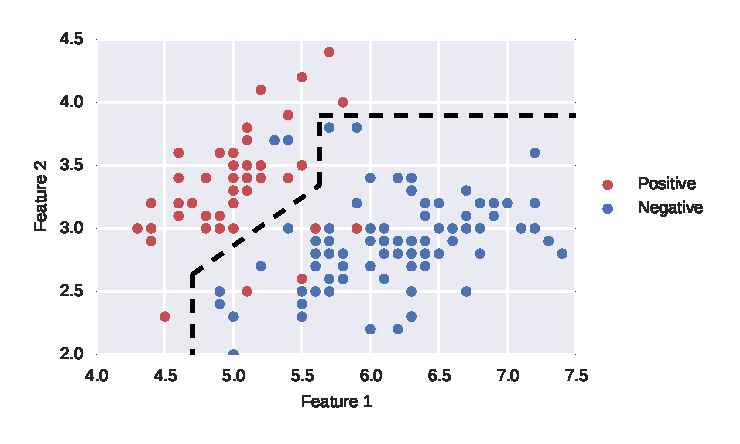
\includegraphics{ch2_fig2}
	\caption{Example of a classification algorithm. Using a set of examples from two classes, a 
	classification algorithm is learn in order to separate between the positives and the negatives. }
	\label{fig:ch2:2}
\end{figure}

    	\begin{table}[!t]
		\centering
		\footnotesize
    \begin{tabular}{c|c|c}
      \multicolumn{3}{c}{}\\
			\multicolumn{1}{c|}{}  & Actual Positive& Actual Negative \\
			\multicolumn{1}{c|}{} & $y=1$& $y=0$ \\
			\hline
			Predicted Positive 		& \multirow{ 2}{*}{37} & \multirow{ 
			2}{*}{2} \\
			$c=1$ & &\\
			\hline
			Predicted Negative  	& \multirow{ 2}{*}{4} & \multirow{ 
			2}{*}{70} \\
			$c=0$ & &\\
		\end{tabular}
		\caption{Confusion matrix of the toy example}
		\label{tab:ch2:2}
  \end{table}  
  Error = 5.31\%
  
\subsection{Families of binary classifiers}
% \subsection{Linear models}
% \subsection{Decision tree models}
% \subsection{Neural networks}
% \subsection{Suport vector machines}
% \subsection{Ensemble based classifiers}
% \section{Sampling}
% \subsection{Under/over sampling}
% \subsection{SMOTE}

% \chapter{Cost-sensitive classification}
% 
% \begin{remark}{Outline}
% \todo{fix outline}
% In this chapter, we present the well-known family of \textit{random forests}
% methods. In Section~\ref{sec:4:bias-variance}, we first describe the bias-variance
% decomposition of the prediction error and then present, in
% Section~\ref{sec:4:ensemble}, how aggregating randomized models through
% ensembles reduces the prediction error by decreasing the variance term in this
% decomposition. In Section~\ref{sec:4:random-forests}, we revisit random forests
% and its variants and study how randomness introduced into the decision trees
% reduces prediction errors by decorrelating the decision
% trees in the ensemble. Properties and features of random forests are then outlined
% in Section~\ref{sec:4:features} while their consistency
% is finally explored in Section~\ref{sec:4:consistency}.
% \end{remark}


\section{Cost-sensitive classification}
\todo{ Change notation}
  Classification, in the context of machine learning, deals with the problem of predicting the class
  of a set of examples given their features. Traditionally, classification methods aim at 
  minimizing the misclassification of examples, in which an example is misclassified if the 
  predicted class is different from the true class. Such a traditional framework assumes that all 
  misclassification errors carry the same cost. This is not the case in many real-world 
  applications. Methods that use different misclassification costs are known as cost-sensitive 
  classifiers. Typical cost-sensitive approaches assume a constant cost for each type of error, in 
  the sense that, the cost depends on the class and is the same among examples 
  \citep{Elkan2001,Kim2012}. 
  Although, this class-dependent approach is not realistic in many real-world applications, for 
  example in credit card fraud detection, failing to detect a fraudulent transaction may have an 
  economical impact from a few to thousands of Euros, depending on the particular transaction and 
  card holder \citep{Sahin2013}. In churn modeling, a model is used for predicting which
  customers are more likely to abandon a service provider. In this context, failing to identify a 
  profitable or unprofitable churner have a significant different financial impact 
  \citep{Glady2009}. Similarly, in direct marketing, wrongly predicting that a customer will not 
  accept an offer when in fact he will, has a different impact than the other way around 
  \citep{Zadrozny2003}. Also in credit scoring, where declining good customers has a non constant 
  impact since not all  customers generate the same profit \citep{Verbraken2014}. Lastly, in the 
  case of intrusion   detection, classifying a benign connection as malicious have a different cost 
  than when a   malicious connection is accepted \citep{Ma2011}.

  In order to deal with these specific types of cost-sensitive problems, called example-dependent
  cost-sensitive, some methods have been proposed recently. However, the literature on 
  example-dependent cost-sensitive methods is limited, mostly because there is a lack of publicly 
  available datasets that fit the problem \citep{MacAodha2013}. Standard solutions consist in 
  modifying the training set by re-weighting the examples proportionately to the misclassification 
  costs \citep{Elkan2001,Zadrozny2003}.

\subsection{Binary classification cost characteristic}
    In classification problems with two classes $y_i \in \{0,1\}$, the objective is to learn or 
    predict to which class $c_i \in \{0,1\}$ a given example $i$ belongs based on its $k$ features 
    $X_i=[x^1_i, x^2_i,...,x^k_i]$. In this context, classification costs can be represented using 
    a 2x2 cost matrix \citep{Elkan2001}, that introduces the costs associated with two types of 
    correct classification, true positives ($C_{TP_i}$), true negatives ($C_{TN_i}$), and the two 
    types of misclassification errors, false positives ($C_{FP_i}$), false negatives ($C_{FN_i}$),
    as defined below:
    \begin{table}[h]
      \caption{Classification cost matrix}
      \centering
      \begin{tabular}{c|c|c}
        \multicolumn{1}{c|}{}  & Actual Positive& Actual Negative \\
        \multicolumn{1}{c|}{} & $y_i=1$& $y_i=0$ \\
        \hline
        Predicted Positive    & \multirow{ 2}{*}{$C_{TP_i}$} & \multirow{ 2}{*}{$C_{FP_i}$} \\
        $c_i=1$ & &\\
        \hline
        Predicted Negative    & \multirow{ 2}{*}{$C_{FN_i}$} & \multirow{ 2}{*}{$C_{TN_i}$} \\
        $c_i=0$ & &\\
      \end{tabular}
    \end{table}  

  Conceptually, the cost of correct classification should always be lower than the cost of 
misclassification.
  These are referred to as the ``reasonableness`` conditions \citep{Elkan2001}, and are defined as
  $C_{FP_i} > C_{TN_i}$ and $C_{FN_i} > C_{TP_i}$.
  Taking into account the ``reasonableness`` conditions, a simpler cost matrix 
  with only one degree of freedom has been defined in \citep{Elkan2001},
  by scaling and shifting the initial cost matrix, resulting in:
  \begin{center}
  \begin{tabular}{c|c}

  \multirow{ 2}{*}{Negative} & \multirow{ 
2}{*}{$C^*_{FN_i}=\frac{(C_{FN_i}-C_{TN_i})}{(C_{FP_i}-C_{TN_i})}$} \\
  \\
  \hline
  \multirow{ 2}{*}{Positive} & \multirow{ 
2}{*}{$C^*_{TP_i}=\frac{(C_{TP_i}-C_{TN_i})}{(C_{FP_i}-C_{TN_i})}$} \\
  \\ 
  \end{tabular}
\end{center}

  A classification problem is said to be cost-insensitive if costs of both errors are equal. It 
    is class-dependent cost-sensitive if the costs are different but constant. Finally we talk 
    about an example-dependent cost-sensitive classification problem if the cost matrix is not 
    constant for all the examples.
  
    However, the definition above is not general enough. There are many cases when the cost matrix 
    is not constant and still the problem is cost-insensitive or class-dependent cost-sensitive. 
    For example, if the costs of correct classification are zero, \mbox{$C_{TP_i}=C_{TN_i}=0$}, 
    and the costs of misclassification are $C_{FP_i}=a_0\cdot z_i$ and $C_{FN_i}=a_1\cdot z_i$,
    where $a_0$, $a_1$, are constant and $z_i$ a random variable. This is an example of a cost 
    matrix that is not constant. However, $C^*_{FN_i}$ and $C^*_{TP_i}$ are constant, i.e. 
    $C^*_{FN_i}=(a_1\cdot z_i)/(a_0\cdot z_i)=a_1/a_0$ and $C^*_{TP_i}=0$ $\forall i$. In 
    this case the problem is cost-insensitive if $a_0=a_1$, or class-dependent cost-sensitive if 
    $a_0 \ne a_1$, even given the fact that the cost matrix is not constant.
  
    Nevertheless, using only the simpler cost matrix is not enough to define when a problem is 
    example-dependent cost-sensitive. To achieve this, we define the classification problem cost 
    characteristic as 
    \begin{equation}
     b_i = C^*_{FN_i}-C^*_{TP_i},
    \end{equation}
    and define its mean and standard deviation as $\mu_b$ and $\sigma_b$, respectively.
  
    Using $\mu_b$ and $\sigma_b$, we analyze different binary classification problems. In the case 
    of a cost-insensitive classification problem, for every example $i$ \mbox{$C_{FP_i}=C_{FN_i}$}
    and $C_{TP_i}=C_{TN_i}$, leading to $b_i=1$ $\forall i$ or more generally $\mu_b=1$ and 
    $\sigma_b=0$. For class-dependent cost-sensitive problems, the costs are not equal but 
    constants \mbox{$C_{FP_i}\ne C_{FN_i}$} or \mbox{$C_{TP_i}\ne C_{TN_i}$}, leading to $b_i \ne 
    1$ $\forall i$, or $\mu_b \ne 1$ and $\sigma_b=0$. Lastly, in the case of example-dependent 
    cost-sensitive problems, the cost difference is non constant or $\sigma_b \ne 0$.
  
    In summary a binary classification problem is defined according to the following conditions:
    \begin{table}[h]
      \centering
      \begin{tabular}{c | c | l}
        $\mu_b$ & $\sigma_b$ & Type of classification problem \\
        \hline 
        && \\
        $1$ &  $0$ & cost-insensitive \\ &&\\
        $\ne 1$ & $0$ & class-dependent cost-sensitive \\ &&\\
        & $\ne 0$ & example-dependent cost-sensitive \\ 
      \end{tabular}
    \end{table}

\subsection{Example-dependent Cost-based evaluation masures}
    Common cost-insensitive evaluation measures such as misclassification rate or \mbox{$F-Score$}, 
    assume the same cost for the different misclassification errors. Using these measures is not 
    suitable for example-dependent cost-sensitive binary classification problems. Indeed, two 
    classifiers with equal misclassification rate but different numbers of false positives and 
    false negatives do not have the same impact on cost since \mbox{$C_{FP_i}\ne C_{FN_i}$};
    therefore there is a need for a measure that takes into account the actual costs 
    ~$C_i=[C_{TP_i},C_{FP_i},C_{FN_i},C_{TN_i}]$ of each example $i$, as introduced in 
    the previous section.
  
    Let $S$ be a set of $N$ examples $i$, $N=\vert S \vert$, where each example is represented by 
    the augmented feature vector \mbox{$X^a_i=[X_i, C_i]$} and labelled using the class label $y_i 
    \in \{0,1\}$.
    A classifier $f$ which generates the predicted label $c_i$ for each element $i$ is trained 
    using the set $S$. Then the cost of using $f$ on $S$ is calculated by
    \begin{align}\label{eq:cost}
      Cost(f(S)) = \sum_{i=1}^{N} & {\bigg( y_i(c_i C_{TP_i} + (1-c_i)C_{FN_i})} + \\
      & {(1-y_i)(c_i C_{FP_i} + (1-c_i)C_{TN_i}) \bigg)}.
    \end{align}

However, the total cost may not be easy to interpret. In \citep{Whitrow2008}, a 
  \textit{normalized} cost measure was proposed, by dividing the total cost by the theoretical 
  maximum cost, which is the cost of misclassifying every example. The \textit{normalized} cost is 
  calculated using
  \begin{align}\label{eq:ncost}
    NCost(f(\mathcal{S})) = \frac{Cost(f(\mathcal{S}))}
    {\sum_{i \in \mathcal{S}_0} C_{FN_i} + 
    \sum_{i \in \mathcal{S}_1} C_{FP_i}},
  \end{align} 
  
  We proposed similar approach in \citep{CorreaBahnsen2014b}, where the savings of using an 
  algorithm  are defined as the cost of the algorithm versus the cost of using no algorithm at all. 
  To do that, the cost of the costless class is defined as 
  \begin{equation}
    Cost_l(\mathcal{S}) = \min \{Cost(f_0(\mathcal{S})), Cost(f_1(\mathcal{S}))\},
  \end{equation}
  where 
  \begin{equation}\label{eq:f_a}
    f_a(\mathcal{S}) = \mathbf{a}, \text{ with } a\in \{0,1\}.
  \end{equation}

  The cost improvement can be expressed as the cost savings as compared with $Cost_l(\mathcal{S})$. 
  \begin{equation}\label{eq:savings}
    Savings(f(\mathcal{S})) = \frac{ Cost_l(\mathcal{S}) - Cost(f(\mathcal{S}))}
    {Cost_l(\mathcal{S})}.
  \end{equation} 


\subsection{State-of-the-art methods}
\todo{Extend description of each method}

    As mentioned earlier, taking into account the different costs associated with each example, 
    some methods have been proposed to make classifiers example-dependent cost-sensitive. These 
    methods may be grouped in two categories. Methods based on changing the class distribution of 
    the training data, which are known as cost-proportionate sampling methods; and direct cost 
    methods \citep{Wang2013}.
  
    A standard method to introduce example-dependent costs into classification algorithms is to 
    re-weight the training examples based on their costs, either by cost-proportionate 
    rejection-sampling \citep{Zadrozny2003}, or over-sampling \citep{Elkan2001}. The 
    rejection-sampling approach consists in selecting a random subset $S_{r}$  by randomly 
    selecting examples from $S$, and accepting each example $i$ with probability $w_i/ 
    \max\limits_{1,\dots, N}\{w_i\}$, where $w_i$ is defined as the expected misclassification 
    error of example $i$:
    \begin{equation}\label{eq_pred1}
      w_i = y_i\cdot C_{FN_i}+(1-y_i)\cdot C_{FP_i}.
    \end{equation}
    Lastly, the over-sampling method consists in creating a new set $S_{o}$, by making $w_i$ 
    copies of each example $i$. However, cost-proportionate over-sampling increases the training 
    since $\vert S_{o}\vert >> \vert S \vert$, and it also may result in over-fitting 
    \citep{Drummond2003}. Furthermore, none of these methods uses the full cost matrix but only the 
    misclassification costs.

In addition to the traditional aforementioned algorithms we also evaluate a thresholding 
optimization to make the 
   classifiers cost sensitive, based on the method proposed in \cite{Sheng2006}.
   The idea behind this approach is to adaptively modify the probability threshold of an 
   algorithm such that a certain criterion is minimized; in our case the cost due to fraud.
   By default the probability threshold of an algorithm is 50\%, meaning that when the probability 
   of a positive event is greater than 50\% that example is classified as positive.
   This default threshold is not necessarily the one that minimizes the cost due to fraud. 
   %So we make an optimization, in the training dataset, in order to find the threshold which 
minimizes the cost measure,
   %and by doing so, we make the algorithm cost sensitive.
   So we make an optimization in the training dataset, in order to find the threshold which 
minimizes the cost measure.
   Then, this new threshold is applied to the test dataset to obtain the results,
   and by doing so, we make the algorithm cost sensitive by threshold optimization.

\chapter{Cost-sensitive classification}\label{ch:3}

\begin{remark}{Outline}
In this chapter, we introduce classifications models from a machine learning perspective. 
Moreover, we present the example-dependent cost-sensitive framework that is the basis of the 
thesis. In Section~\ref{sec:3:classification}, we give a self contain introduction to 
classification, including the most-common algorithms, and the main methods for evaluating the 
performance of the different algorithm. Then, in Section~\ref{sec:3:cs}, we present the general 
framwork of cost-sensitive classification. Within this Section, we first introduce a method for 
defining the type of cost-sensitivity of a problem. Afterwards, we present the different 
cost-sensitive performance evaluation measures. Lastly, we show the state-of-the-art 
example-dependent cost-sensitive methods cost-proportionate rejection-sampling and 
cost-proportionate over-sampling.
\end{remark}


\section{Introduction}
\label{sec:3:intro}

  Classification, in the context of machine learning, deals with the problem of predicting the class
  of a set of examples given their features. Traditionally, classification methods aim at 
  minimizing the misclassification of examples, in which an example is misclassified if the 
  predicted class is different from the true class. Such a traditional framework assumes that all 
  misclassification errors carry the same cost. This is not the case in many real-world 
  applications. Methods that use different misclassification costs are known as cost-sensitive 
  classifiers. Typical cost-sensitive approaches assume a constant cost for each type of error, in 
  the sense that, the cost depends on the class and is the same among examples
  \citep{Elkan2001,Kim2012}. Although, this class-dependent approach is not realistic in many 
  real-world applications.
  
  \begin{remark}{Real-world cost sensitive applications}
  For example in credit card fraud detection, failing to detect a fraudulent transaction may have 
  an economical impact from a few to thousands of Euros, depending on the particular transaction 
  and card holder \citep{Sahin2013}. In churn modeling, a model is used for predicting which
  customers are more likely to abandon a service provider. In this context, failing to identify a 
  profitable or unprofitable churner have a significant different financial impact 
  \citep{Glady2009}. Similarly, in direct marketing, wrongly predicting that a customer will not 
  accept an offer when in fact he will, has a different impact than the other way around 
  \citep{Zadrozny2003}. Also in credit scoring, where declining good customers has a non constant 
  impact since not all  customers generate the same profit \citep{Verbraken2014}. Lastly, in the 
  case of intrusion   detection, classifying a benign connection as malicious have a different cost 
  than when a   malicious connection is accepted \citep{Ma2011}.
  \end{remark}

  In order to deal with these specific types of cost-sensitive problems, called example-dependent
  cost-sensitive, some methods have been proposed recently. However, the literature on 
  example-dependent cost-sensitive methods is limited, mostly because there is a lack of publicly 
  available datasets that fit the problem \citep{MacAodha2013}. Standard solutions consist in 
  modifying the training set by re-weighting the examples proportionately to the misclassification 
  costs \citep{Elkan2001,Zadrozny2003}.

  
\section{Class-dependent cost-sensitive classification}
\label{sec:3:class-dependent}

The cost-sensitive literature is mostly focused in class-dependent problems \citep{Elkan2001}, where 
the cost of misclassification is associated with the class. Ussually, the cost of misclassifying a 
positive example is denoted by $c_0$ and the one of misclassifying a negative example is denoted by 
$c_1$. Conceptually, $c_0\ge0$ and $c_1\ge0$, moreover, it is ussually defined that $c_0+c_1=2$ 
\citep{Flach2011a}, as when $c_0=c_1=1$ represents the case of cost-insensitive classification. 
Using the previous notation, a class-dependent cost measure is defined as \citep{Wang2014}:
\begin{equation}
  Cost_{cd}(f(\mathcal{S})) = c_0 \cdot FP + c_1 \cdot FN,
\end{equation}
where $FP$ and $FN$ are the number of false positives and false negatives, respectively.

Following the toy example shown in Section~\ref{sec:2:classification}, we now assume that 
misclassifying a negative example have a cost of $c_0=0.2$ and a positive example $c_1=1.8$. 
Under this scenario, the misclassifying a positive example have a much higher cost than 
misclassifying a negative one. Taking that into account, in \figurename{~\ref{fig:3:1}, we show an 
algorithm (Algorithm3), that focus on maximizing the correct classification of the positives, 
scarifying the correct classification of the negatives. In the following table, we compare the 
results of the standard measures and the class-dependent cost, of Algorithm3 and the classification 
algorithms presented in \figurename{~\ref{fig:2:2b}} (Algorithm1) and \figurename{ \ref{fig:2:3}} 
(Algorithm2):
\begin{center}
    \footnotesize
  \begin{tabular}{l|c|c|c|c|c}
  Algorithm & Error & Recall & Precision & $F_1Score$ & $Cost_{cd}$ \\
  \hline
  Algorithm1 & 11.11\% & 87.8\%& 90\%& 88.8\% & 9.8\\ %FP = 4 , FN=5
  Algorithm2 & 5.3\% & 90.2\%& 94.9\%& 92.5\% & 7.6\\ %FP = 2 , FN=4
  Algorithm3 & 7.97\%& 92.68\% &86.36\%& 89.41\% & 6.6 \\
  \end{tabular}
\end{center}

\begin{figure}[t!]
  \centering
  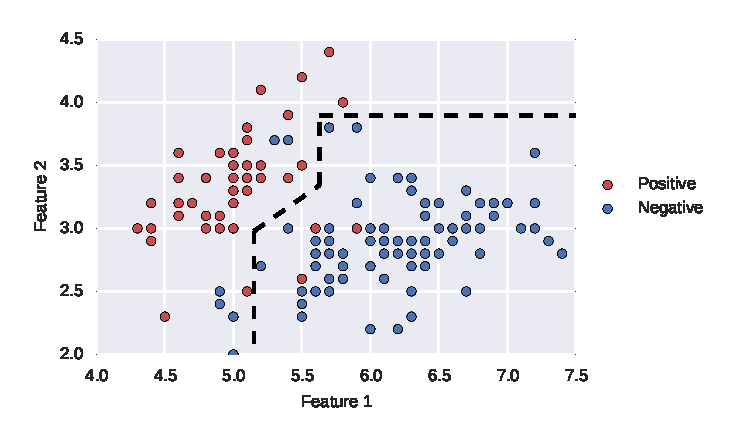
\includegraphics{ch3_fig1}
  \caption{Class-dependent cost-sensitive classification algorithm. Since the cost of misclassifying 
positives and negatives is different, the algorithm focus on maximizing the correct classification 
of the positives, scarifying the correct classification of the negatives.}
  \label{fig:3:1}
\end{figure}

It is found, that by focusing on the positives, Algorithm3 arises to a lower cost, even though, the 
traditional metrics are worst than Algorithm2. In conclusion, it is of highly importance to take 
into account the cost when evaluating and training a classification model.


\section{Example-dependent cost-sensitive classification}

The class-dependent framework introduced in the previous section, is highly restrictive, as 
assuming that the different costs are constant between classes is not realistic in many real world 
applications. In fraud detection, fraudulent transactions  can have a financial impact from 
hundreds or thousands of Euros \cite{Sahin2013}.


\section{Binary classification cost characteristic}
\label{sec:3:cost_characteristic}

  In classification problems with two classes $y_i \in \{0,1\}$, the objective is to learn or 
  predict to which class $c_i \in \{0,1\}$ a given example $i$ belongs based on its $k$ features 
  $\mathbf{x}_i=[x^1_i, x^2_i,...,x^k_i]$. In this context, classification costs can be 
  represented using a 2x2 cost matrix \citep{Elkan2001}, that introduces the costs 
  associated with   two types of correct   classification, true positives ($C_{TP_i}$), true 
  negatives ($C_{TN_i}$),   and the two  types of   misclassification errors, false positives 
  ($C_{FP_i}$), false negatives   ($C_{FN_i}$), as   defined in \tablename{ 
  \ref{tab:3:cost_matrix}}.

  
  \begin{table}[t]
    \centering
    \footnotesize
    \begin{tabular}{c|c|c}
      \multicolumn{1}{c|}{}  & Actual Positive& Actual Negative \\
      \multicolumn{1}{c|}{} & $y_i=1$& $y_i=0$ \\
      \hline
      Predicted Positive    & \multirow{ 2}{*}{$C_{TP_i}$} & \multirow{ 2}{*}{$C_{FP_i}$} \\
      $c_i=1$ & &\\
      \hline
      Predicted Negative    & \multirow{ 2}{*}{$C_{FN_i}$} & \multirow{ 2}{*}{$C_{TN_i}$} \\
      $c_i=0$ & &\\
    \end{tabular}
    \caption{Classification cost matrix}
    \label{tab:3:cost_matrix}
  \end{table}  

  Conceptually, the cost of correct classification should always be lower than the cost of 
  misclassification. These are referred to as the ``reasonableness`` conditions \citep{Elkan2001}, 
  and are defined as  $C_{FP_i} > C_{TN_i}$ and $C_{FN_i} > C_{TP_i}$.
  Taking into account the ``reasonableness`` conditions, a simpler cost matrix 
  with only one degree of freedom has been defined in \citep{Elkan2001},
  by scaling and shifting the initial cost matrix, resulting in:
  \begin{center}
    \footnotesize
    \begin{tabular}{c|c}
    \multirow{ 2}{*}{Negative} & \multirow{ 
    2}{*}{$C^*_{FN_i}=\frac{(C_{FN_i}-C_{TN_i})}{(C_{FP_i}-C_{TN_i})}$} \\
    \\
    \hline
    \multirow{ 2}{*}{Positive} & \multirow{ 
    2}{*}{$C^*_{TP_i}=\frac{(C_{TP_i}-C_{TN_i})}{(C_{FP_i}-C_{TN_i})}$} \\
    \\ 
    \end{tabular}
  \end{center}

  A classification problem is said to be cost-insensitive if costs of both errors are equal. It 
  is class-dependent cost-sensitive if the costs are different but constant. Finally we talk 
  about an example-dependent cost-sensitive classification problem if the cost matrix is not 
  constant for all the examples.

  However, the definition above is not general enough. There are many cases when the cost matrix 
  is not constant and still the problem is cost-insensitive or class-dependent cost-sensitive. 
  For example, if the costs of correct classification are zero, $C_{TP_i}=C_{TN_i}=0$, 
  and the costs of misclassification are $C_{FP_i}=a_0\cdot z_i$ and $C_{FN_i}=a_1\cdot z_i$,
  where $a_0$, $a_1$, are constant and $z_i$ a random variable. This is an example of a cost 
  matrix that is not constant. However, $C^*_{FN_i}$ and $C^*_{TP_i}$ are constant, i.e. 
  $C^*_{FN_i}=(a_1\cdot z_i)/(a_0\cdot z_i)=a_1/a_0$ and $C^*_{TP_i}=0$ $\forall i$. In 
  this case the problem is cost-insensitive if $a_0=a_1$, or class-dependent cost-sensitive if 
  $a_0 \ne a_1$, even given the fact that the cost matrix is not constant.

  Nevertheless, using only the simpler cost matrix is not enough to define when a problem is 
  example-dependent cost-sensitive. To achieve this, we proposed in \citep{CorreaBahnsen2015}, 
  the classification problem cost characteristic as:
  \begin{equation}
    b_i = C^*_{FN_i}-C^*_{TP_i},
  \end{equation}
  and define its mean and standard deviation as $\mu_b$ and $\sigma_b$, respectively.

  Using $\mu_b$ and $\sigma_b$, we analyze different binary classification problems. In the case 
  of a cost-insensitive classification problem, for every example $i$ \mbox{$C_{FP_i}=C_{FN_i}$}
  and $C_{TP_i}=C_{TN_i}$, leading to $b_i=1$ $\forall i$ or more generally $\mu_b=1$ and 
  $\sigma_b=0$. For class-dependent cost-sensitive problems, the costs are not equal but 
  constants \mbox{$C_{FP_i}\ne C_{FN_i}$} or \mbox{$C_{TP_i}\ne C_{TN_i}$}, leading to $b_i \ne 
  1$ $\forall i$, or $\mu_b \ne 1$ and $\sigma_b=0$. Lastly, in the case of example-dependent 
  cost-sensitive problems, the cost difference is non constant or $\sigma_b \ne 0$.

  In summary a binary classification problem is defined according to the following conditions:
  \begin{center}
    \footnotesize
    \begin{tabular}{c | c | l}
      $\mu_b$ & $\sigma_b$ & Type of classification problem \\
      \hline 
      && \\
      $1$ &  $0$ & cost-insensitive \\ &&\\
      $\ne 1$ & $0$ & class-dependent cost-sensitive \\ &&\\
      & $\ne 0$ & example-dependent cost-sensitive \\ 
    \end{tabular}
  \end{center}
  

\subsection{Example-dependent evaluation measures}
\label{sec:3:csmeasures}

  Common cost-insensitive evaluation measures such as misclassification rate or \mbox{$F_1Score$}, 
  assume the same cost for the different misclassification errors. Using these measures is not 
  suitable for example-dependent cost-sensitive binary classification problems. Indeed, two 
  classifiers with equal misclassification rate but different numbers of false positives and 
  false negatives do not have the same impact on cost since \mbox{$C_{FP_i}\ne C_{FN_i}$};
  therefore there is a need for a measure that takes into account the actual costs 
  $\{C_{TP_i},C_{FP_i},C_{FN_i},C_{TN_i}\}$ of each example $i$, as introduced in the previous 
  Section.
  \label{ntn:ch2:3}

  Let $\mathcal{S}$ be a set of $N$ examples $i$, $N=\vert S \vert$, where each example is 
  represented by  the augmented feature vector $\mathbf{x}_i^*=[\mathbf{x}_i, 
  C_{TP_i},C_{FP_i},C_{FN_i},C_{TN_i}]$  and labeled using the class   label $y_i   \in \{0,1\}$. 
  A classifier $f$ which generates the   predicted label $c_i$ for each   element $i$ is trained  
  using the set $\mathcal{S}$. Then the cost of   using $f$ on $\mathcal{S}$ is calculated by
  \begin{equation}\label{eq:3:cost_total}
     Cost(f(\mathcal{S})) = \sum_{i=1}^N Cost(f(\mathbf{x}_i^*)),
  \end{equation}
  where
   \begin{align}\label{eq:3:cost}
    Cost(f(\mathbf{x}_i^*)) =& y_i(c_i C_{TP_i} + (1-c_i)C_{FN_i}) + \nonumber \\  
    & (1-y_i)(c_i C_{FP_i} + (1-c_i)C_{TN_i}).
  \end{align}

  However, the total cost may not be easy to interpret. In \citep{Whitrow2008}, a 
  \textit{normalized} cost measure was proposed, by dividing the total cost by the theoretical 
  maximum cost, which is the cost of misclassifying every example. The \textit{normalized} cost is 
  calculated using
  \begin{align}\label{eq:3:ncost}
    Cost_n(f(\mathcal{S})) = \frac{Cost(f(\mathcal{S}))}
    {\sum_{i=1}^N C_{FN_i} \cdot \mathbf{1}_0(y_i) 
    +  C_{FP_i} \cdot \mathbf{1}_1(y_i)  }.
  \end{align} 

  We proposed similar approach in \citep{CorreaBahnsen2014b}, where the savings of using an 
  algorithm  are defined as the cost of the algorithm versus the cost of using no algorithm at all. 
  To do that, the cost of the costless class is defined as 
  \begin{equation}
    Cost_l(\mathcal{S}) = \min \{Cost(f_0(\mathcal{S})), Cost(f_1(\mathcal{S}))\},
  \end{equation}
  where 
  \begin{equation}\label{eq:3:f_a}
    f_a(\mathcal{S}) = \mathbf{a}, \text{ with } a\in \{0,1\}.
  \end{equation}

  The cost improvement can be expressed as the cost savings as compared with $Cost_l(\mathcal{S})$. 
  \begin{equation}\label{eq:3:savings}
    Savings(f(\mathcal{S})) = \frac{ Cost_l(\mathcal{S}) - Cost(f(\mathcal{S}))}
    {Cost_l(\mathcal{S})}.
  \end{equation} 


\subsection{State-of-the-art methods}

  As mentioned earlier, taking into account the different costs associated with each example, 
  some methods have been proposed to make classifiers example-dependent cost-sensitive. These 
  methods may be grouped in two categories. Methods based on changing the class distribution of 
  the training data, which are known as cost-proportionate sampling methods; and direct cost 
  methods \citep{Wang2013}.

  A standard method to introduce example-dependent costs into classification algorithms is to 
  re-weight the training examples based on their costs, either by cost-proportionate 
  rejection-sampling \citep{Zadrozny2003}, or over-sampling \citep{Elkan2001}. The 
  rejection-sampling approach consists in selecting a random subset $\mathcal{S}_{r}$  by 
  randomly  selecting examples from $\mathcal{S}$, and accepting each example $i$ with 
  probability $w_i/ \max\limits_{1,\dots, N}\{w_i\}$, where $w_i$ is defined as the expected 
  misclassification error of example $i$:
  \begin{equation}\label{eq_pred1}
    w_i = y_i\cdot C_{FN_i}+(1-y_i)\cdot C_{FP_i}.
  \end{equation}
  Lastly, the over-sampling method consists in creating a new set $\mathcal{S}_{o}$, by making 
  $w_i$ copies of each example $i$. However, cost-proportionate over-sampling increases the 
  training  since $\vert \mathcal{S}_{o}\vert >> \vert \mathcal{S} \vert$, and it also may result 
  in over-fitting  \citep{Drummond2003}. Furthermore, none of these methods uses the full cost 
  matrix but only the  misclassification costs.

  The second approach, consists in using the predicted probability $\hat p_i$, estimated using a 
  given classifier $f$, and   modify the threshold $t$  such that the savings are maximized. 
  This method is called cost-sensitive thresholding \citep{Sheng2006}. The idea behind this 
approach 
  is to adaptively modify the probability threshold of an algorithm $f_t$ in order to maximized the 
  savings of the algorithm on a given set $Savings(f^t(\mathcal{S}))$. The threshold is calculated 
  using the following equation
  \begin{equation}
   t_{thresholding} = \argmax_t Savings(f^t(\mathcal{S})).
  \end{equation}

  